\chapter{Facility design}
    Since there was no existing LSP facility at McGill University, a considerable portion of this project revolved around the design and fabrication of an LSP generator. This chapter will discuss the major design requirements of such a system, the selection of appropriate solutions, and the assembly, integration, and testing process. Several practical issues were encountered in developing the LSP generator, which are rarely mentioned in the experimental LSP literature. They will be documented in detail in this report in the hopes that this can facilitate future work in this field.

    \section{Needs and requirements}


        \begin{statement}{Need statement} 
            In order to properly define the problem solved by a system, a need statement is needed.
        \end{statement}

        \subsection{Existing hardware}
            The laser made available for this project was the most important driver of many design decisions. Wether they are for interstellar-class lightsails as envisioned by \textcite{lubinRoadmapInterstellarFlight2022}, or interplanetary missions powered by electric propulsion as proposed by \textcite{sheerinFastSolarSystem2021}, fiber lasers operating at the 1064-nm-wavelength are currently favored for many DEP applications. Since LTP is proposed as an additional DEP concept within this ecosystem, this experimental work aimed to match this laser wavelength.

            An IPG Photonics YLR-300/3000-QCW-MM-AC Ytterbium fiber laser (seen in \autoref{fig:laser_laser}) was generously loaned to the IFERG by the Royal Military College of Canada. This is an infrared laser primarily designed for welding, drilling, and cutting. It is capable of operating in both pulsed and continuous modes at a wavelength of \qty{1070}{nm}. Its key specifications are summarized in \autoref{tab:laser_spec}. A complete calibration report for the laser can be found in \autoref{chp:app_YLR}. An IPG Photonics P30-001736 collimator head (seen in \autoref{fig:laser_collimator}) was also acquired for the laser, forming a 13.6-mm-diameter beam at its output. The collimator's calibration report can be found in \autoref{chp:app_Collimator}.

            Although a practical LTP system would likely operate in continuous mode, the YLR laser's pulsed mode was of particular interest in this project. As discussed in \autoref{sec:background_lsp}, laser power is a critical factor in the ability to achieve a steady LSP. The YLR laser is not only capable of pulsing at an order of magnitude above its CW power rating, but it is able to do so for several milliseconds, a relatively long-pulse in the world of laser physics. This pulse is in fact so long that it is considered to be in the CW regime as far as laser damage is concerned (\textcite{thorlabsNBK7PlanoConvexLenses}), hence the \emph{Quasi}-Continuous-Wave (QCW) designation of this laser. This capability enables running very high power experiments without investing in far more expensive (and dangerous) CW kW-class lasers, though the 10~ms timescale imposes a major constraint on the facility design and experimental methodology.
        
            \begin{table}
                \centering
                \caption{Summary of nominal laser specifications}
                \label{tab:laser_spec}
                \begin{tabular}{@{}lrl@{}}
                    \toprule
                    \textbf{Parameter}            & \textbf{Quantity} & \textbf{Unit} \\ \midrule
                    Wavelength                    & 1070              & nm            \\
                    Maximum CW Power              & 300               & W             \\
                    Maximum Pulse Power           & 3000              & W             \\
                    Maximum Pulse Duration (3 kW) & 10                & ms            \\
                    Maximum Pulse Energy          & 30              & J             \\ \bottomrule
                    \end{tabular}
            \end{table}

            \begin{figure}[h]
                \centering
                \begin{subfigure}[t]{0.6\textwidth}
                    \centering
                    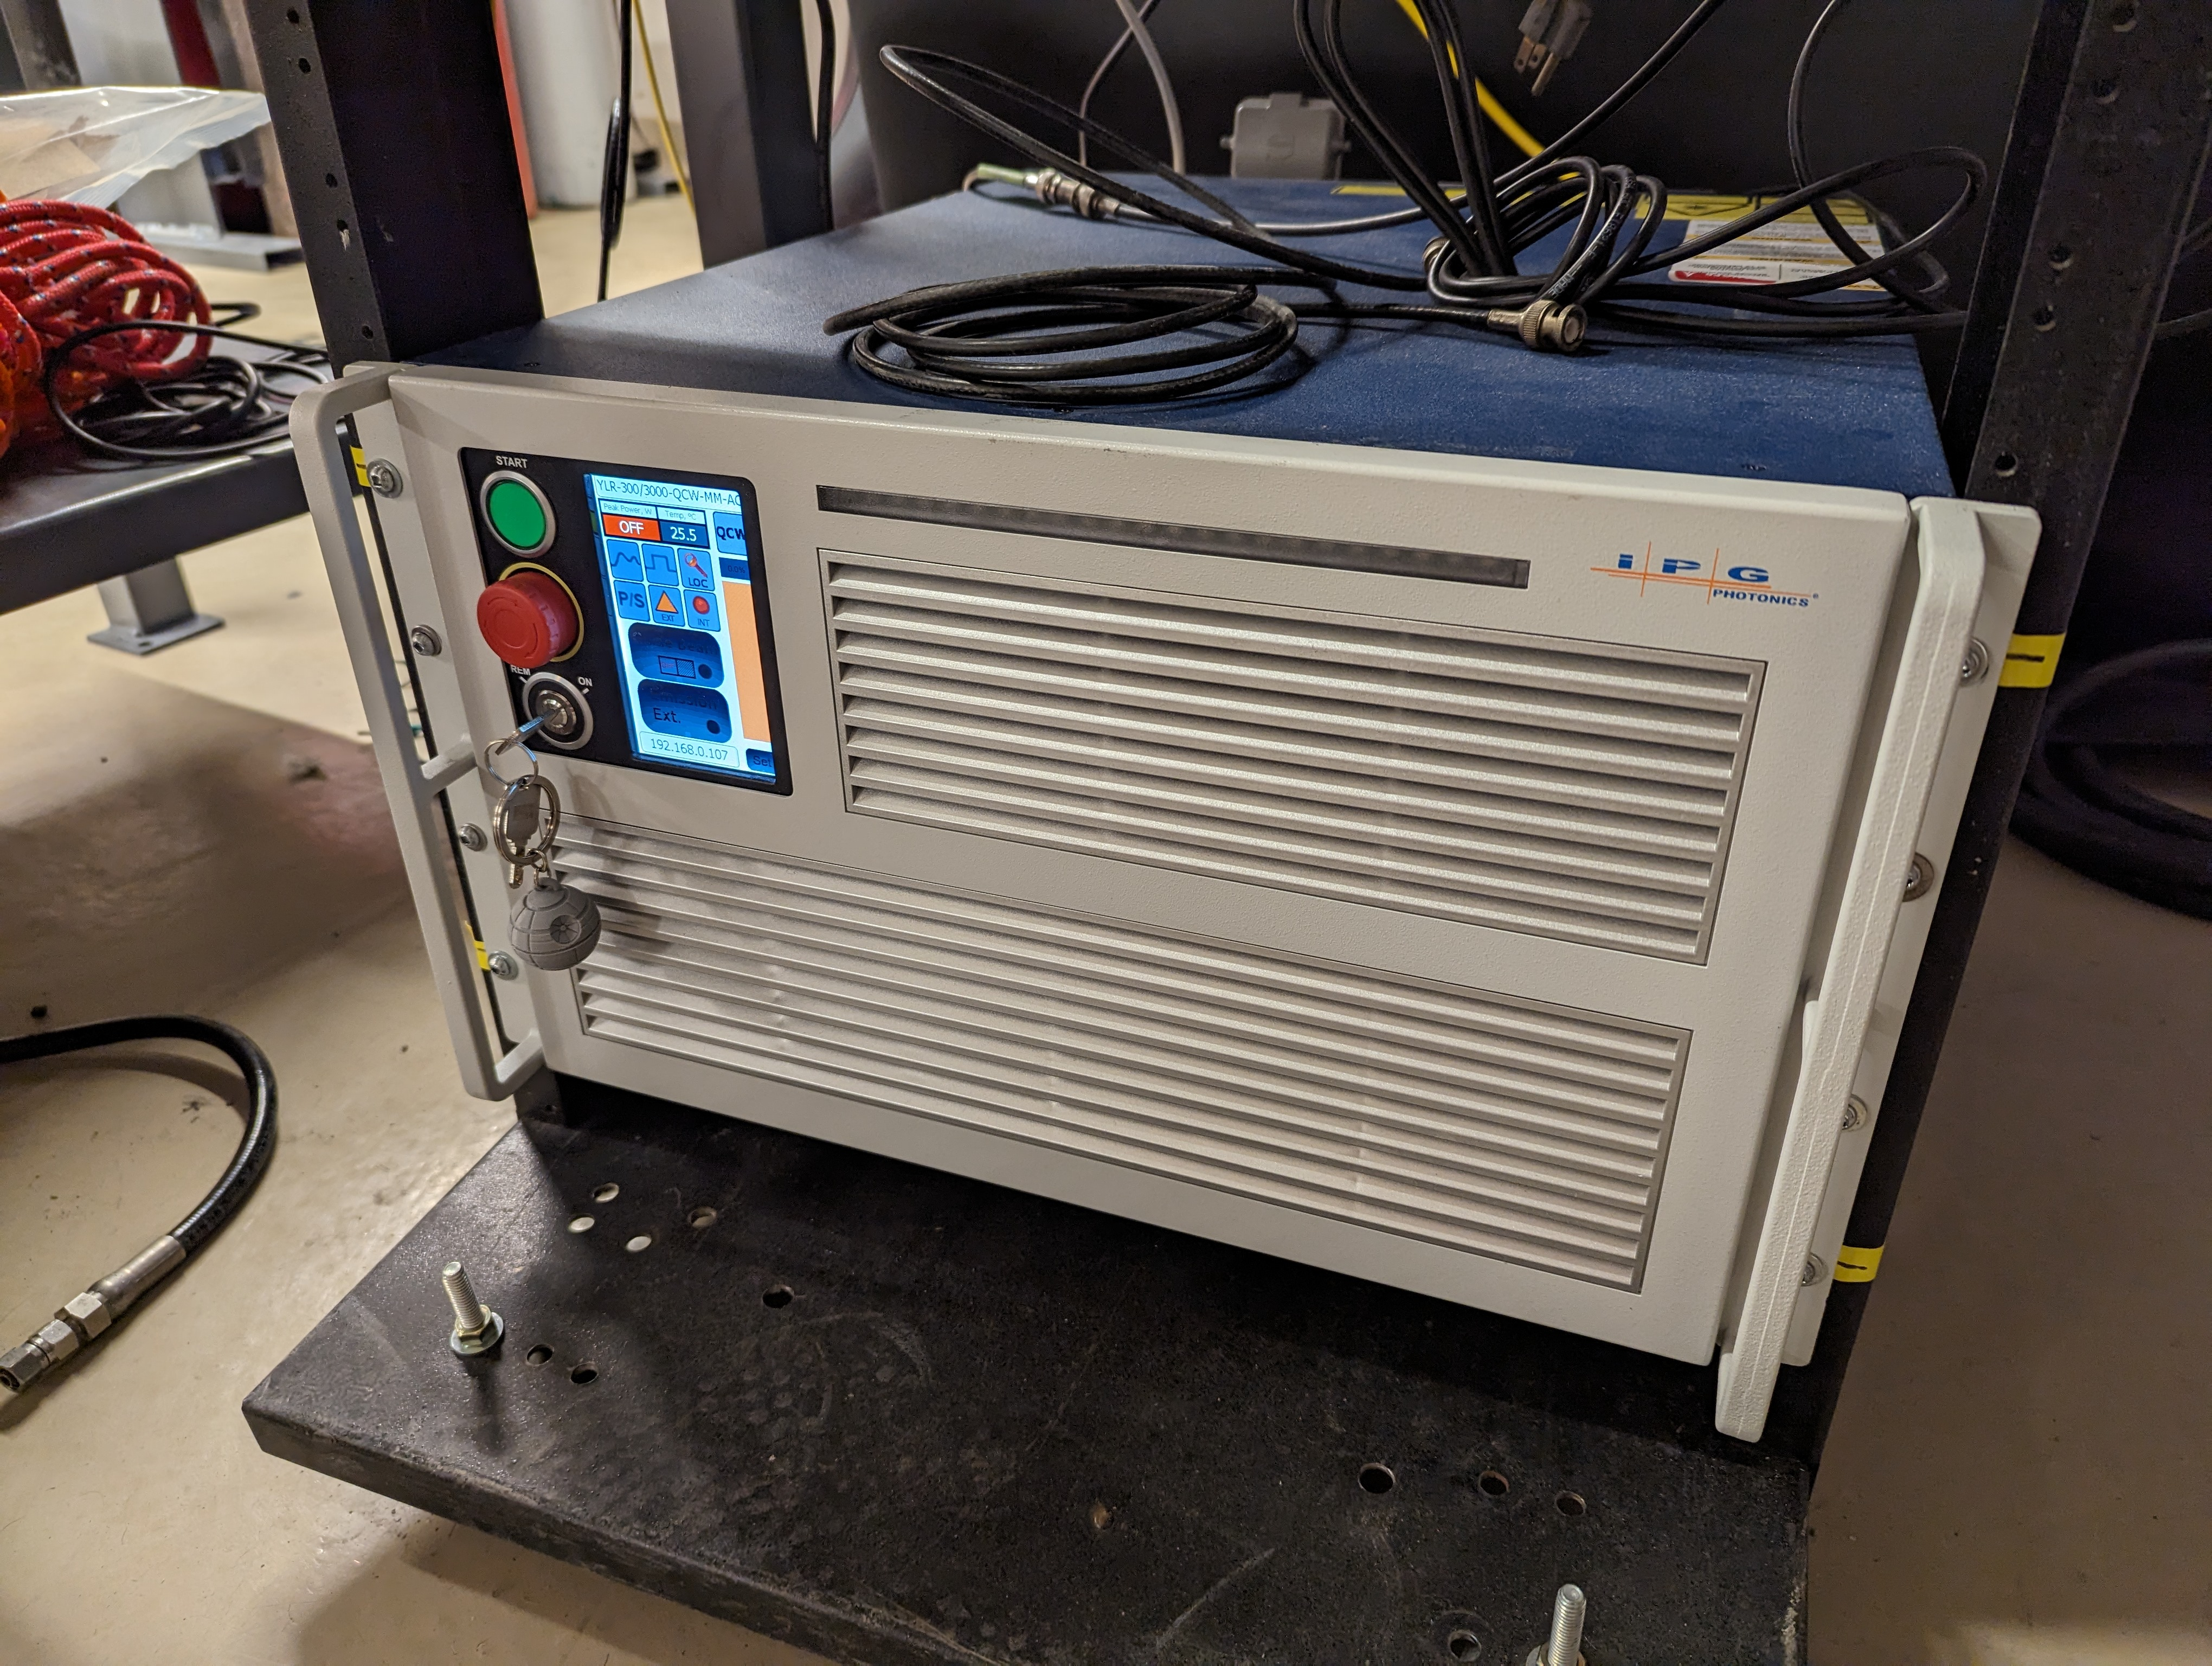
\includegraphics[height=2.6in]{assets/3 design/laser.jpg}
                    \caption{IPG Photonics YLR-300/3000-QCW-MM-AC Laser}
                    \label{fig:laser_laser}
                \end{subfigure}
                \begin{subfigure}[t]{0.35\textwidth}
                    \centering
                    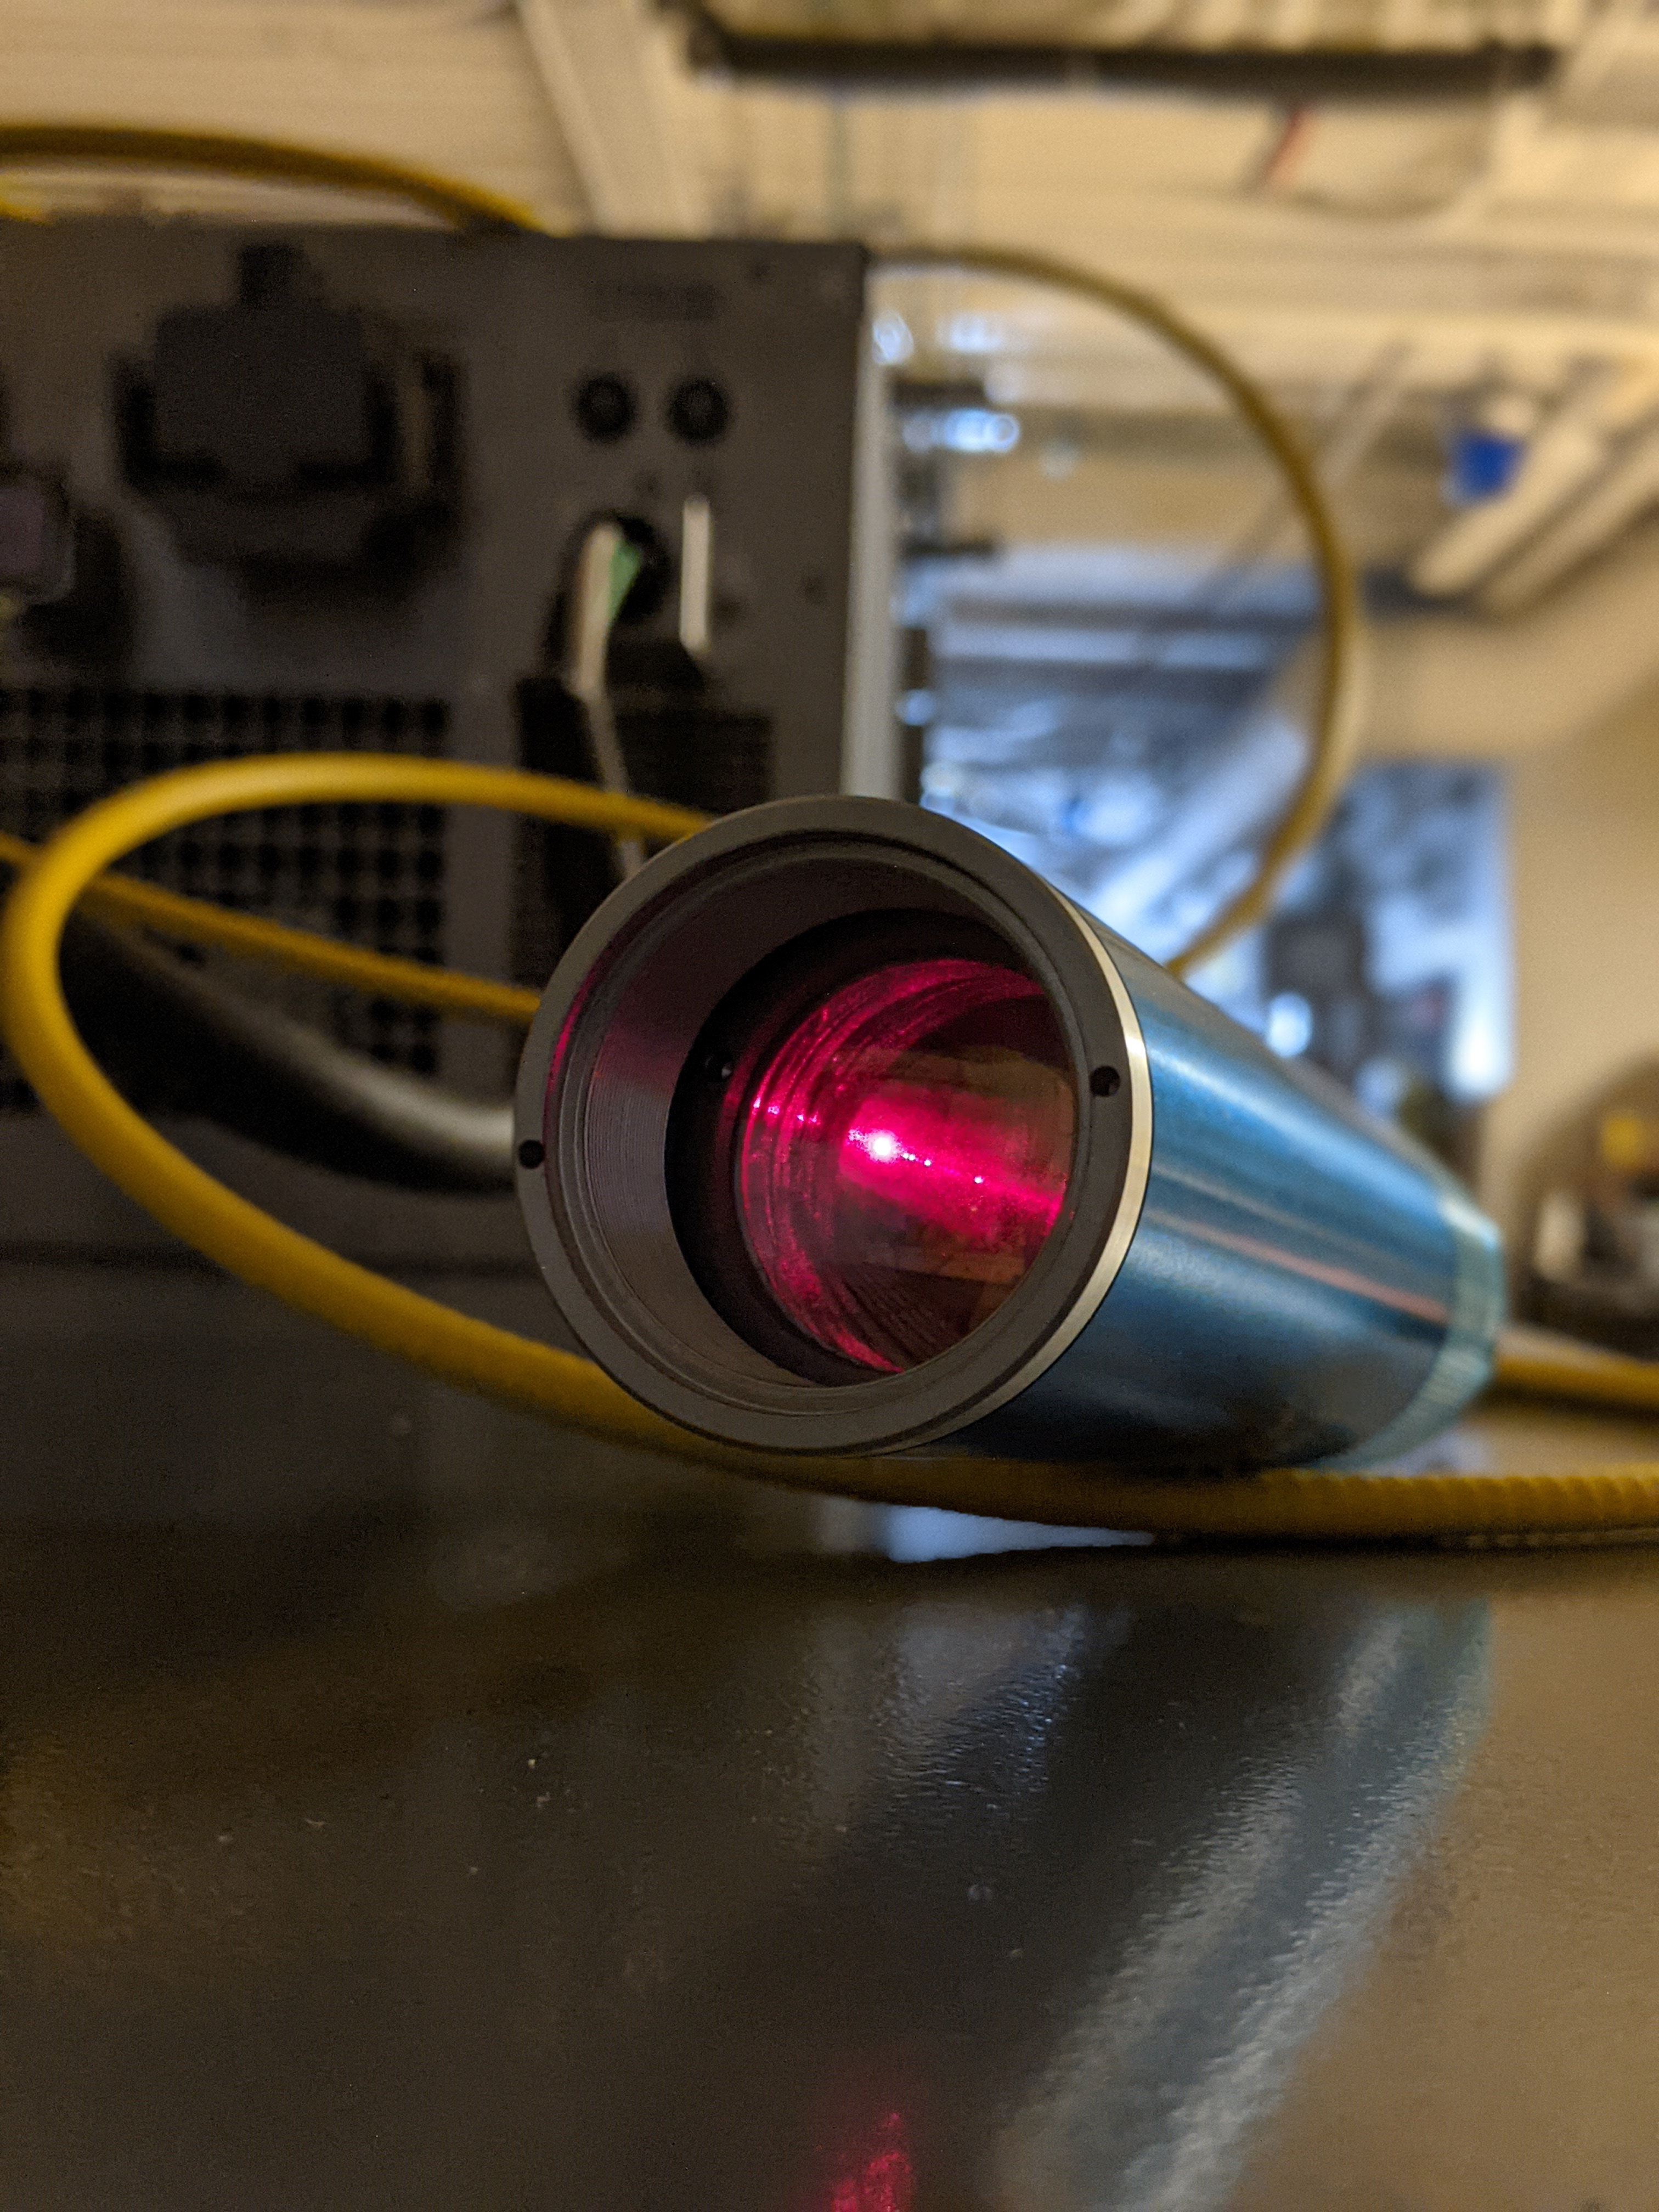
\includegraphics[height=2.6in]{assets/3 design/collimator_r.jpg}
                    \caption{Laser collimator head}
                    \label{fig:laser_collimator}
                \end{subfigure}
                \caption{Laser system used for this project}
                \label{fig:laser}
            \end{figure}

        \subsection{Requirements}

            \begin{table}[h]
                \renewcommand{\arraystretch}{1.3}
                \centering
                \caption{Top-level design requirements for the LTP laboratory model (the ``thruster'')}
                \label{tab:lttmReq}
                \begin{tabular}{l>{\raggedright}p{0.4\textwidth}p{0.4\textwidth}<{\raggedright}}
                    \toprule
                    \textbf{Identifier}  & \textbf{Requirement}   & \textbf{Rationale} \\
                    \midrule
                    LTTLM-1     & The thruster shall operate at a maximum laser power of \qty{3}{kW} at a wavelength of \qty{1070}{nm}    & This is the laser system made available for this experiment \\
                    LTTLM-2     & The thruster shall operate using gaseous argon at room temperature as a propellant & The past experiments used for comparison also used argon \\
                    LTTLM-3     & The thruster shall operate at a maximum design pressure of 2~\unit{MPa} & This should allow the generation of LSP even in continuous-wave laser modes \\
                    LTTLM-4     & The thruster shall allow visible observation of the LSP in the thrust chamber & This enables high-speed imaging of the plasma and the remote measurement of its temperature \\
                    LTTLM-5     & The thruster shall provide chamber pressure and gas temperature data   & This permits the estimation of stagnation conditions for the heated propellant \\
                    LTTLM-6     & The thruster shall allow the measurement of absorbed laser power   & This is one of the major energy losses to be determined \\
                    \bottomrule
                \end{tabular}
            \end{table}

    \section{Design process}
        \subsection{Test section}
            The requirements for the Laser-Thermal Thruster Laboratory Model (LTTLM) are listed in \autoref{tab:lttmReq}. In summary, the thruster model should be a pressurized vessel featuring one or more windows to allow laser input and optical viewing of the LSP. Furthermore, this vessel should allow the integration of various instrumentation systems. The design and manufacture of such a vessel would have required a significant amount of time, so the alternative of re-purposing hardware from a different project was considered first. This hardware's specifications could be compared to the requirements, and modifications could be made if necessary.

            Coincidentally, \textcite{kokkalisOnsetCavitationDynamically2023} at the neighboring McGill Fluid Dynamics Lab was undertaking research into cavitation effects within piston-cylinder assemblies. Their apparatus included cylindrical sections designed to withstand high dynamic pressures encountered in their experiments, and featured windows or transparent walls to track the onset of cavitation with high-speed cameras. The design was modular, allowing the installation of various endcaps with different functions. This theoretically fulfilled requirements LTTLM\nobreakdash-2 to LTTLM\nobreakdash-4. One particular test section (pictured in \autoref{fig:cavitation}, detailed drawings can be found in \autoref{chp:app_CavitatorDrawings}) had been fabricated with a set of instrumentation ports and polycarbonate windows spanning the length of the cylinder. This test section had been tested in a few experiments but was found to be inadequate, as gaps around the ports and windows were sources of parasitic cavitation.

            \begin{figure}[h]
                \centering
                \begin{subfigure}[t]{0.46\textwidth}
                    \centering
                    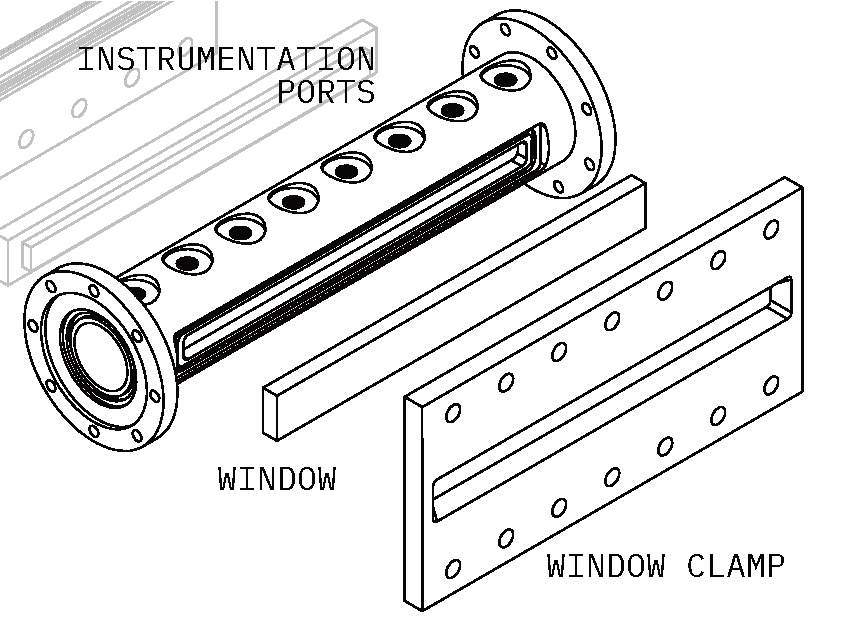
\includegraphics[width=\textwidth]{assets/3 design/cavitatorDrawing.pdf}
                    \caption{Assembly schematic}
                    \label{fig:cavitation_schematic}
                \end{subfigure}
                \begin{subfigure}[t]{0.49\textwidth}
                    \centering
                    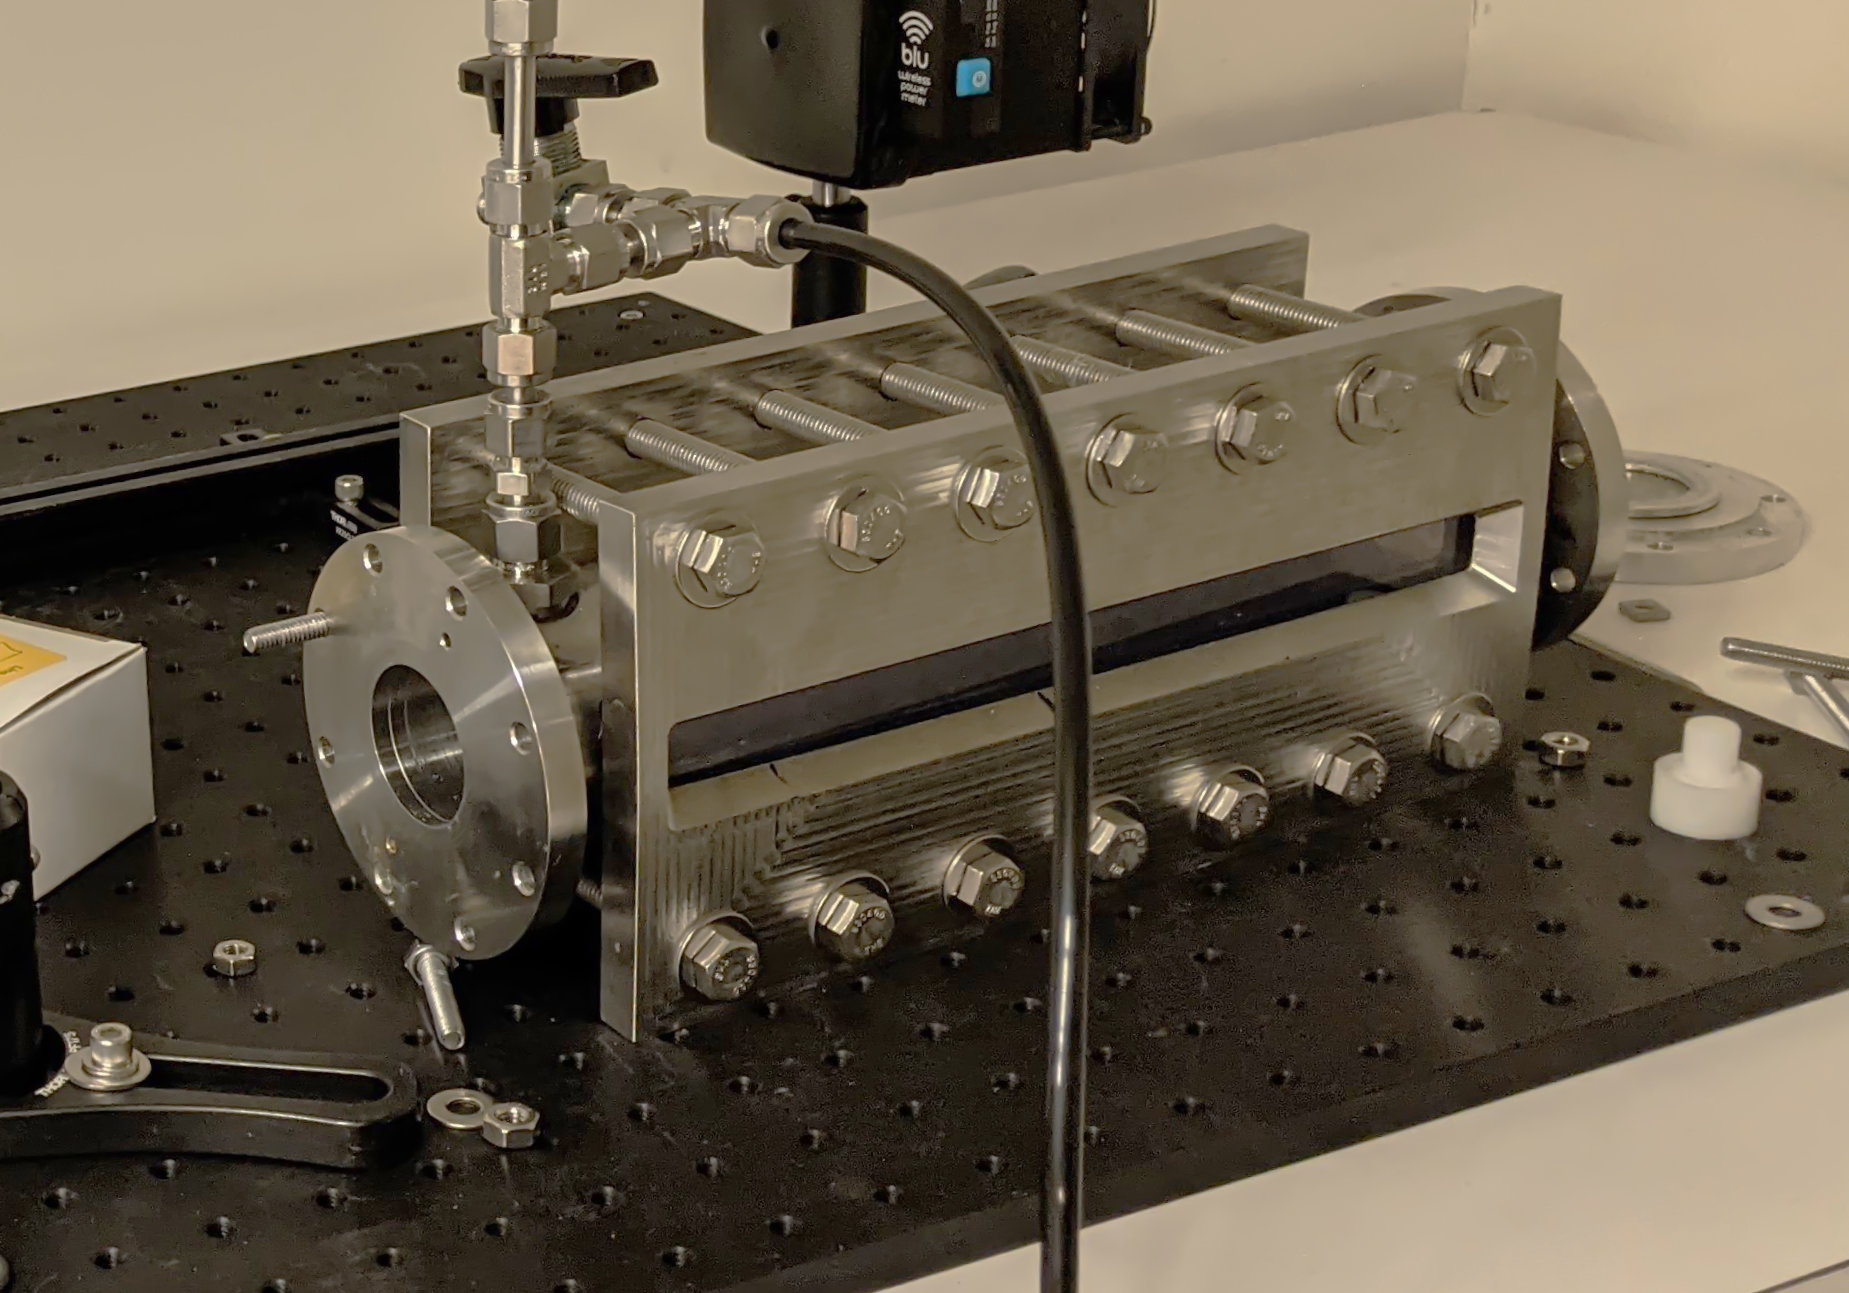
\includegraphics[width=\textwidth]{assets/3 design/cavitationSection.jpg}
                    \caption{Photograph of the test section fitted with a gas feed line}
                    \label{fig:cavitation_photo}
                \end{subfigure}
                \caption{Cavitation test section}
                \label{fig:cavitation}
            \end{figure}

            As seen in \autoref{tab:lttmReq_partialVerif}, this apparatus was verified against the requirements set in \autoref{tab:lttmReq} to determine what retro-fitting activities would be needed to use it as an LTP thruster model. It was found that very little retrofitting work was required in order to use it as an LSP generator: special instrument plugs could be created, and special laser window endcaps were needed to seal the apparatus while allowing the laser to enter the test section. To operate the system as a thruster, a separate nozzle endcap could be made. Finally, as spectrometry was planned to be used for plasma temperature determination, the polycarbonate side windows would have to be exchanged for UV-grade quartz windows, which would allow a broader spectrum of radiation to pass through.
            
            However, using this test section would not come without a set of drawbacks. Its original intent made it unoptimized to work as a laser-thermal thruster model for the following reasons:
            \begin{enumerate}
                \item Though its thick stainless steel construction made it very safe for the operating pressures of the project, it also made it heavy. The superfluous mass would make frictional loads on a thrust bench far more significant than for a custom-designed, lightweight thruster model.
                \item Its length forces the use of long focal-length lenses to focus the laser into the test section. Such long lenses would create a high {\itshape f}-number beam, which could affect how easily a stable LSP could be achieved, as discussed in \autoref{sec:background_lsp}. While shorter lenses would still be able to focus the laser into the chamber, the beam past the focal point would diverge quickly and hit the test section walls, affecting laser absorption measurements at best, or damaging experimental apparatus at worst.
                \item Instrumentation ports are available only on one side of the cylinder. The lack of opposing ports constrains the design of certain ignition methods, such as spark igniters.
            \end{enumerate}



            \begin{table}[h]
                \renewcommand{\arraystretch}{1.3}
                \centering
                \caption{Verification of LTTLM requirements for the cavitation apparatus}
                \label{tab:lttmReq_partialVerif}
                \begin{tabular}{l>{\raggedright}p{0.53\textwidth}p{0.27\textwidth}<{\raggedright}}
                    \toprule
                    \textbf{Identifier} & \textbf{Requirement}                                                                   & \textbf{Status}                   \\ \midrule
                    LTTLM-1             & The thruster shall operate at a maximum laser power of \qty{3}{kW} at a wavelength of \qty{1070}{nm} & Requires laser windows            \\
                    LTTLM-2             & The thruster shall operate using gaseous argon at room temperature as a propellant     & Fulfilled                         \\
                    LTTLM-3             & The thruster shall operate at a maximum design pressure of 2 MPa                       & Fulfilled                         \\
                    LTTLM-4             & The thruster shall allow visible observation of the LSP in the thrust chamber          & Fulfilled                         \\
                    LTTLM-5             & The thruster shall provide chamber pressure and gas temperature data                   & Requires special instrument plugs \\
                    LTTLM-6             & The thruster shall allow the measurement of absorbed laser power                       & Requires laser windows            \\ \bottomrule
                \end{tabular}
            \end{table}

    \section{Integration and test}